% Rational points on the unit circle from Hilbert's Theorem 90. Generated by a short script.
\begin{tikzpicture}[font=\small,scale=2.4]
\draw[gray,->] (-1.25,0) -- (1.3,0); \draw[gray,->] (0,-0.2) -- (0,1.2);
\draw[thick,MidnightBlue] (1,0) arc (0:180:1);
\draw[BrickRed!40] (-1,0) -- (0.0000,1.0000);
\draw[BrickRed!40] (-1,0) -- (-0.6000,0.8000);
\draw[BrickRed!40] (-1,0) -- (-0.8000,0.6000);
\draw[BrickRed!40] (-1,0) -- (-0.8824,0.4706);
\draw[BrickRed!40] (-1,0) -- (0.6000,0.8000);
\draw[BrickRed!40] (-1,0) -- (-0.3846,0.9231);
\draw[BrickRed!40] (-1,0) -- (0.8000,0.6000);
\draw[BrickRed!40] (-1,0) -- (0.3846,0.9231);
\draw[BrickRed!40] (-1,0) -- (-0.2800,0.9600);
\draw[BrickRed!40] (-1,0) -- (0.8824,0.4706);
\draw[BrickRed!40] (-1,0) -- (0.2800,0.9600);
\fill[BrickRed] (0.0000,1.0000) circle (0.6pt);
\fill[BrickRed] (-0.6000,0.8000) circle (0.6pt);
\fill[BrickRed] (-0.8000,0.6000) circle (0.6pt);
\fill[BrickRed] (-0.8824,0.4706) circle (0.6pt);
\fill[BrickRed] (-0.9231,0.3846) circle (0.6pt);
\fill[BrickRed] (-0.9459,0.3243) circle (0.6pt);
\fill[BrickRed] (-0.9600,0.2800) circle (0.6pt);
\fill[BrickRed] (0.6000,0.8000) circle (0.6pt);
\fill[BrickRed] (-0.3846,0.9231) circle (0.6pt);
\fill[BrickRed] (-0.7241,0.6897) circle (0.6pt);
\fill[BrickRed] (-0.8491,0.5283) circle (0.6pt);
\fill[BrickRed] (0.8000,0.6000) circle (0.6pt);
\fill[BrickRed] (0.3846,0.9231) circle (0.6pt);
\fill[BrickRed] (-0.2800,0.9600) circle (0.6pt);
\fill[BrickRed] (-0.4706,0.8824) circle (0.6pt);
\fill[BrickRed] (-0.6897,0.7241) circle (0.6pt);
\fill[BrickRed] (0.8824,0.4706) circle (0.6pt);
\fill[BrickRed] (0.2800,0.9600) circle (0.6pt);
\fill[BrickRed] (-0.2195,0.9756) circle (0.6pt);
\fill[BrickRed] (-0.5077,0.8615) circle (0.6pt);
\fill[BrickRed] (0.9231,0.3846) circle (0.6pt);
\fill[BrickRed] (0.7241,0.6897) circle (0.6pt);
\fill[BrickRed] (0.4706,0.8824) circle (0.6pt);
\fill[BrickRed] (0.2195,0.9756) circle (0.6pt);
\fill[BrickRed] (-0.1803,0.9836) circle (0.6pt);
\fill[BrickRed] (-0.3243,0.9459) circle (0.6pt);
\fill[BrickRed] (0.9459,0.3243) circle (0.6pt);
\fill[BrickRed] (0.1803,0.9836) circle (0.6pt);
\fill[BrickRed] (-0.1529,0.9882) circle (0.6pt);
\fill[BrickRed] (0.9600,0.2800) circle (0.6pt);
\fill[BrickRed] (0.8491,0.5283) circle (0.6pt);
\fill[BrickRed] (0.6897,0.7241) circle (0.6pt);
\fill[BrickRed] (0.5077,0.8615) circle (0.6pt);
\fill[BrickRed] (0.3243,0.9459) circle (0.6pt);
\fill[BrickRed] (0.1529,0.9882) circle (0.6pt);
\fill (-1,0) circle (0.8pt) node[below] {$-1$};
\draw[->,gray] (1.05,0.95) node[right,black] {$\tfrac35+\tfrac45i=\tfrac{2+i}{2-i}$} -- (0.63,0.81);
\end{tikzpicture}
